\section{Differentialligninger 2}
\begin{enumerate}
	\item Svarene er:
	\begin{align*}
	y(x)=3x+2,&&y(x)=-\cos(x)+3,&&y(x)=-\frac{1}{2}e^{-2x}+\frac{5}{2}.
	\end{align*}
	
	\item Løsningen er
	\begin{align*}
	y(x)=e^{-(x+1)}
	\end{align*}
	som går gennem punktet $(1,\frac{1}{e^2})$. 
	
	\item Tangenten har ligningen $y=\frac{7}{3}(x-1)+3$.

	\item Svarene er
\begin{enumerate}
	\item $y(x)=\frac{3}{4}x^4-x-1$.
	\item $y(x)=\sqrt{2}e^{x}$.
	\item $y(x)=-3e^{-\frac{x}{3}}$.
\end{enumerate}	
	
		\item Tangenten har ligning $y=-22(x-3)+5$
		
		\item\label{it:diffeq21ans} I Figur~\ref{fig:diffeq21ans} ses en skitse af løsningerne til differentialligningen
	\begin{align*}
	y'=x+y,
	\end{align*}
	med begyndelsesbetingelser
	\begin{enumerate}
		\item $y(0)=0$.
		\item $y(0)=-1$.
		\item $y(0)=-2$.
	\end{enumerate}
	
	
	\begin{figure}
		\centering
		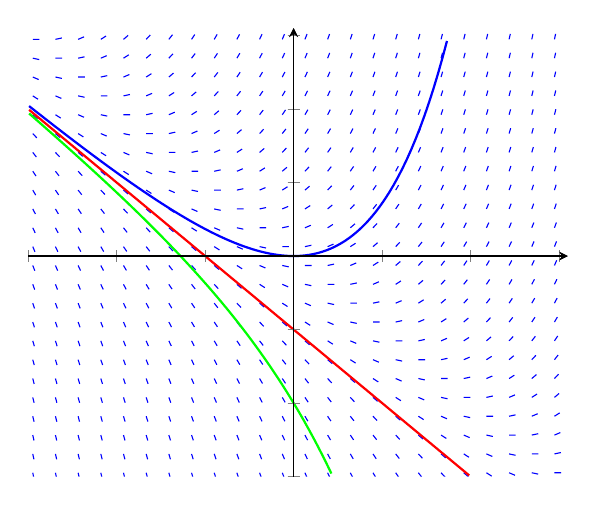
\begin{tikzpicture}[
		declare function={f(\x,\y) = \y+\x;} % Define which function we're using
		]
		\begin{axis}[
		axis x line=center,axis y line=center	,xmin=-3, xmax=3.1, % Axis limits
		ymin=-3, ymax=3.1,view={0}{90},xtick={-3,-2,-1,0,1,2,3}, ytick={-3,-2,-1,0,1,2,3},restrict x to domain=-3:3,restrict y to domain=-3:3]
		\def\length{sqrt(1+(f(x,y)^2)}
		\addplot3[blue, quiver={u={1/(\length)}, v={(f(x,y))/(\length)}, scale arrows=0.075},samples=40] {0};
%		\addplot[thick,black,samples=200] {2*e^x-x-1};
				\addplot[thick,blue,samples=200] {e^x-x-1};
				\addplot[thick, red,samples=200] {-x-1};
				\addplot[thick,green,samples=200] {-e^x-x-1};
		%\addplot {x^2+0.15}; % You need to find the antiderivative yourself, unfortunately. Good exercise!
		\end{axis}
		\end{tikzpicture} 
		\caption{Opgave~\ref{it:diffeq21ans}}
		\label{fig:diffeq21ans}
	\end{figure}
	
		\item Tangenten har ligning $y=2(x-4)+1=2x-7$. 
		
	\item Svarene er:
	\begin{enumerate}
		\item $y(x)=ae^{kx}$.
		\item $y(x)=\frac{b}{k}e^{kx}$.
	\end{enumerate}
	
	
	\item Tangentens har ligning $y= 6(x-1)+4$.	
	
	
	\item Tangenten har ligning $y=3(x-2)+7$.
	
	\item \label{it:diffeq22ans}	I Figur~\ref{fig:diffeq22ans} ses en skitse løsningerne til differentialligningen
	\begin{align*}
	\frac{y'}{y}=x^2-x,
	\end{align*}
	med begyndelsesbetingelser
	\begin{enumerate}
		\item $y(0)=1$.
		\item $y(0)=-1$.
		\item $y(0)=-2$.
	\end{enumerate}
	
	
	\begin{figure}
		\centering
		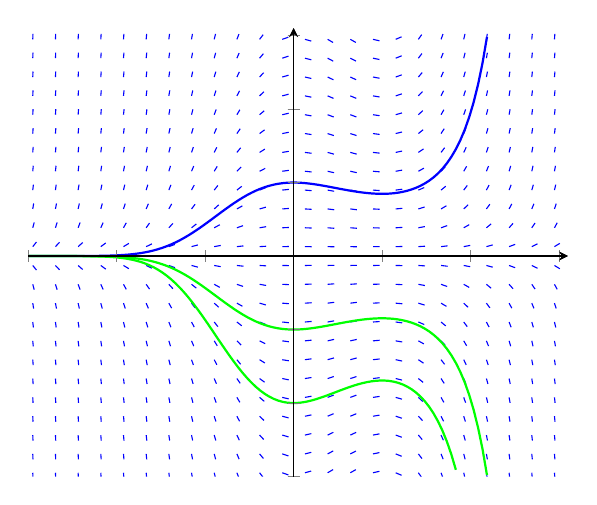
\begin{tikzpicture}[
		declare function={f(\x,\y) = \y*(\x*\x-\x);} % Define which function we're using
		]
		\begin{axis}[
		axis x line=center,axis y line=center	,xmin=-3, xmax=3.1, % Axis limits
		ymin=-3, ymax=3.1,view={0}{90},xtick={-3,-2,-1,0,1,2,3}, ytick={-3,-2,-1,0,1,2,3},restrict y to domain=-3:3]
		\def\length{sqrt(1+(f(x,y)^2)}
		\addplot3[blue, quiver={u={1/(\length)}, v={(f(x,y))/(\length)}, scale arrows=0.075},samples=40] {0};
%		\addplot[thick,black,samples=200] {2*e^(x^2*(2*x-3)/6)};
		\addplot[thick,blue,samples=200] {1*e^(x^2*(2*x-3)/6)};
		%\addplot[thick, red,samples=200] {0*e^(x^2*(2*x-3)/6)};
		\addplot[thick,green,samples=200] {-1*e^(x^2*(2*x-3)/6)};
		\addplot[thick,green,samples=200] {-2*e^(x^2*(2*x-3)/6)};
		%\addplot {x^2+0.15}; % You need to find the antiderivative yourself, unfortunately. Good exercise!
		\end{axis}
		\end{tikzpicture}
		\caption{Opgave~\ref{it:diffeq22ans}}
		\label{fig:diffeq22ans}
	\end{figure}
	
	
	
	\item Vi har at 
	\begin{align*}
	g'(x)=\frac{d}{dx}(F(x)-F(x_0))=F'(x)=f(x),
	\end{align*}
	samt $g(x_0)=y_0$.
	
	
	
	
	
	
	
\end{enumerate}